
% This is LLNCS.DOC the documentation file of
% the LaTeX2e class from Springer-Verlag
% for Lecture Notes in Computer Science, version 2.4
\documentclass{llncs}
\usepackage{llncsdoc}
\usepackage{color}
\usepackage{graphicx}
\usepackage{listings, tikz, xcolor}
\usepackage{bold-extra}
\usepackage{subfig}
\usepackage{enumerate}
\usepackage[backgroundcolor=pink!40, disable]{todonotes}
\usepackage{courier}
\usepackage{syntax}
\usepackage{amsmath}
\usepackage{hyperref}
\usepackage{MnSymbol}
%
\lstset{ 
	language = [AspectJ]Java,
  basicstyle=\sffamily\small,
  numbers=left,
	numberstyle=\tiny\color[rgb]{0.25,0.25,0.25},
	numberblanklines=false,
  firstnumber=auto,
	breaklines=true,
  tabsize=2,
	emph={aspect,declare, adapter, instance, pointcut, adaptee, adapts, select, UNTIL,pc, instanceType, exp, removeExp, subsetof, supersetof}, 
	emphstyle=\textbf,
	stringstyle=\textsf,
	showstringspaces= false,
	frame=single,
	captionpos = b,
	numberbychapter=false,
	breakatwhitespace = true
	}
\lstset{prebreak=\raisebox{0ex}[0ex][0ex]{\ensuremath{\rhookswarrow}}} 
%
\begin{document}

\title{Aspect-Oriented Language Mechanisms for Component Binding}

\author{Kardelen Hatun \and Christoph Bockisch \and Mehmet Ak\c{s}it}
\institute{TRESE, University of Twente \\ 7500AE Enschede \\ The Netherlands \\
\url{http://www.utwente.nl/ewi/trese/}\\
\email{ \{hatunk,c.m.bockisch,aksit\}@ewi.utwente.nl}
}


\maketitle 

\begin{abstract}{Domain Specific Languages (DSLs) are programming
languages customized for a problem/solution domain, which allow development of
software modules in high-level specifications. Code generation is a common practice
for making DSL programs executable: A DSL specification is transformed to a functionally equivalent GPL
(general-purpose programming language) representation. Integrating the module
generated from a DSL specification to a base system poses a challenge, especially in a case
where the DSL and the base system are developed independently.
In this paper we describe the problem of integrating domain-specific
modules to a system non-intrusively and promote loose coupling between these to
allow software evolution. We present our on-going work on aspect-oriented language mechanisms for defining object selectors and object adapters as a solution to this problem.}
\end{abstract}

\section{Introduction}
Complex systems are created by assembling software components of various types
and functions. Reuse is essential and
components created for a system are required to continue working after the system has
evolved. Some components may be
domain-specific, meaning their structure and functionality can be defined using
the fundamental concepts of the relevant domains. A domain-specific language
(DSL) provides expressive power over a particular domain. It allows software
development with high-level specifications; if general-purpose programming languages
are used, development may take a considerable programming effort. 

The specifications written in a DSL can be processed in various ways. These are
comprehensively described in \cite{Mernik:whenandhow} and
\cite{fowler2010domain}. Generative programming \cite{Czarnecki:overview} is one
of the processing options and has become highly popular with the emergence of
user-friendly language workbenches. Most language workbenches provide a means
to develop a compiler for the DSL, facilitating code generation in general-purpose
languages. (A comparison matrix for language workbenches can be found in
\cite{LWC}.) 

In this paper we focus on the integration of components into target systems.
``Component'' is a very general concept and it can be realized in different forms,
depending on the system. We particularly focus on a subset of components,
\emph{domain-specific components}, which are instances of domain-specific meta-models.
The component structure is described with a DSL and the semantics are embedded
into code generation templates, which are used to generate a component that is tailored towards a base system's requirements.
  

Integrating a generated component into a system poses three main challenges.
(1) When adding unforeseen functionality to a
system, no explicit \emph{hooks} exist for attaching the
generated component. In this case it may be necessary to modify the
generated code, the system code or both to make the connection, which will
expose the system developer to the implementation details of the generated code.
(2) The interfaces of the generated component and the target system should be compatible to work together, which is generally not the case. Then one of the interfaces should be adapted, possibly by modifying the system's or the component's implementation or their type-system.
(3) When the component or the target system evolves, the links between them
must be re-established. 



Current aspect-oriented languages offer mechanisms to modularly implement solutions for the first challenge. It can be solved by defining pointcuts that are used as hooks to a system. The second challenge is our main focus. Existing AO-languages offer limited mechanisms for implementing adapters between interfaces. AspectJ inter-type declarations can be used to make system classes to implement appropriate interfaces, however this approach is type-invasive. CaesarJ offers a more declarative approach with \emph{wrappers}, but their instantiation requires pointcut declarations or they should be explicitly instantiated in the base system. The links mentioned in the third challenge  are the adapter implementations mentioned in the second challenge and they represent the binding between two components. However current AO languages do not offer a declarative way for describing such a binding; an imperative programming language will lead to less readable and less maintainable implementation, which is fragile against software evolution.

\section{Approach}

In order to overcome the shortcomings of the existing approaches we intend to design a declarative way of implementing object adapters which is used together with a specialized pointcut for selecting objects. The object adapter pattern is common practice for binding two components that have incompatible interfaces. Our approach is aspect-oriented and it will provide the means to non-intrusively define and instantiate object adapters, inside aspects. These adapters represent links between the component and the system; their declarative design requires a declarative way of selecting the adaptee objects. 

In order to select objects to be adapted, we have designed a new pointcut mechanism called \emph{instance pointcut} which selects sets of objects based on the execution history.
An instance pointcut definition consists of three parts: an identifier, a type which is the upper bound for all objects in the selected set, and a specification of relevant objects.
The specification utilizes \emph{pointcut expressions} to select events that define the begin and end of life-cycle phases and to expose the object.
At these events, an object is added or removed from the set representing the instance pointcut.
It is possible to access all objects currently selected by an instance pointcut and to
be notified when an object is added or removed.
New instance pointcuts can be derived from existing ones in several ways. Firstly, a new instance pointcut can be derived from another one by restricting the type of selected objects. Secondly, a \emph{subset} or a \emph{super-set} of an existing instance pointcut can be declared whereby the specification of the life-cycle phase is either narrowed down or broadened. Finally, instance pointcut declarations can be composed arbitrarily by means of boolean operators. 

Adapter declarations refer to the sets selected by instance pointcuts, and automatically instantiate adapters for each object in the referred set. Unlike inter-type declarations, adapter declarations are not type invasive; they are compiled to the object adapter pattern and they do not change the type hierarchy of the contained object. They also do not require explicit instantiations. 

\vspace{-5pt}
\begin{figure}[h]
\subfloat[The shapes hierarchy]{
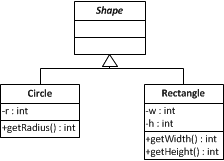
\includegraphics[width=0.27\textwidth]{images/shapes.png}
\label{fig:shapes}
}
\hspace{10pt}
\subfloat[ShapeInfo class that requires two unsupported interfaces]{
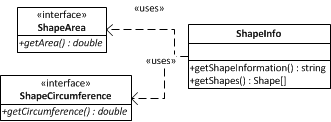
\includegraphics[width=0.55\textwidth]{images/shapeint.png}
\label{fig:shapeint}
}
\caption{Incompatible interfaces: Shape and ShapeInfo}
\label{fig:shapeinfo}
\end{figure}

The header of an adapter declaration consists of an identifier, the list of interfaces the adapter implements and an instance pointcut reference which contains the adaptee objects. In the body of an adapter declaration implementation of the interface methods is provided. In Figure~\ref{fig:shapes} a \textsf{Shape} hierarchy and the interfaces offered by the classes in this hierarchy is shown. The \textsf{ShapeInfo} class uses \textsf{ShapeArea} and \textsf{ShapeCircumference} interfaces to query existing \textsf{Shape}s (Figure~\ref{fig:shapeint}). However none of the classes in the shapes hierarchy implements these interfaces, hence they should be adapted. Assume that there is a class called \textsf{CircleCreator} which has two methods: \textsf{createLargeCircle} and \textsf{createSmallCircle}. We can define an instance pointcut called \textsf{largeCircles} which selects the set of \textsf{Circle} objects that are created by the \textsf{createLargeCircle} method. Here instance pointcuts give us expressive power over selecting specific objects as adaptees. Listing~\ref{circleadapter} shows an example of an adapter declaration. The name of the adapter is \textsf{CircleAdapter} and it implements the interfaces defined in the square brackets; \textsf{CircleAdapter} adapts the objects selected by the \textsf{circles} instance pointcut. In the body of the adapter the implementations of the two declared interfaces are provided. The \textsf{\textbf{adaptee}} keyword refers to an object in the \textsf{circles} set. 

\begin{lstlisting}[float, label={circleadapter}, caption={The adapter declaration for \textsf{Circle} objects}]
declare adapter: CircleAdapter[ShapeArea, ShapeCircumference] adapts largeCircles
{
	public double getArea()
	{
		return Math.pow(adaptee.getRadius(),2)*Math.PI;
	}
	public double getCircumference()
	{
		return 2*adaptee.getRadius()*Math.PI;
	}
}
\end{lstlisting} 

\section{Compilation and Run-time Support}
In our prototype implementation instance pointcuts are compiled to AspectJ and Java code. Roughly, an instance pointcut is transformed into several AspectJ pointcuts, advice declarations, a set structure and methods for altering this set.  Adapter declarations will also be compiled to AspectJ. According to our initial analysis an adapter declaration will map to a Java class for the adapter and advice bodies for initializing adapters. These advice bodies will reference the pointcuts generated from the instance pointcut which is referenced by the adapter declaration. 

We intend to provide run-time support for retrieving adapter instances. Adapters are automatically initialized when an adaptee object satisfying the referenced instance pointcut's conditions become available. These adapter instances can be indexed and accessed through a run-time library. To do this, we have the requirement that the results of a retrieval will always be non-ambiguous e.g. if a query to retrieve a single adapter instance, matches two adapters, then there should be appropriate resolution mechanisms or user feedback to overcome the issue. 






\bibliographystyle{splncs03}{}
\bibliography{main}
\end{document}
